While there are many powerful, widely available, free/libre tools for gathering, manipulating, and analyzing large datasets, CSCW is an interdisciplinary field and  researchers' expertise for using these tools varies quite widely.  Even for researchers with such expertise, the beginning of a large-scale analysis is fraught with technical issues around formatting, types and structure.  This results in a long process of trial and error. For researchers without such expertise, engineering around these problems can be intractable.

For example, at a past OOC data analysis workshop that we organized for the GROUP'15 conference, our expert participants spent the majority of the workshop day (5 hours) converting and loading (100m row) datasets into an analysis framework that would allow the larger group to answer basic questions.  Even after the data was loaded, there were substantial concerns about inconsistencies between the documentation and the observed row counts.

With the goal of democratizing data analysis, we have been experimenting with open dataset interfaces that allow us to do such basic data engineering work up front and minimize the difficulty that future researchers experience when \emph{breaking into} datasets.  We have identified two components that characterize open dataset interfaces: (1) public GUI sandboxes and query interfaces for lightweight, in-situ data exploration and (2) approachable query languages (e.g. SQL).

We have developed such an open dataset interface for Wikimedia datasets in the form of a public SQL querying service: Quarry.  Quarry loads row-based datasets into a relational database management system and allows a user to join and filter datasets on the server through a web-based user interface.  This service allows both the direct download of datasets and download/sharing of secondary datasets produced by queries.  We have found that non-experts can acquire proficiency in SQL over the course of an hour and that experts can use SQL powerfully.  Further, by making past queries public, newcomers are able to observe common and advanced querying strategies on their dataset of interest. This helps non-experts to quickly gain proficiency and, thus, become increasingly comfortable with new technologies that support their research agendas.

\begin{marginfigure}[-35pc]
  \begin{minipage}{\marginparwidth}
    \centering
    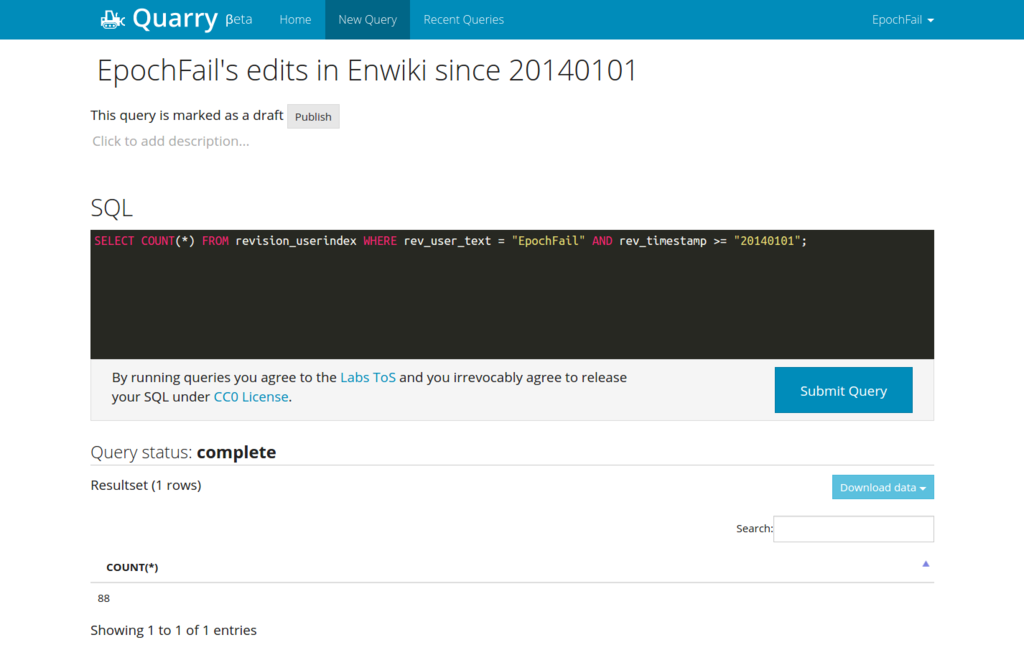
\includegraphics[width=0.9\marginparwidth]{figures/quarry}
    \caption{A screenshot of the Quarry public querying system}~\label{fig:marginfig}
  \end{minipage}
\end{marginfigure}

We see querying interfaces like these as a key opportunity to make OOC datasets more accessible to both data engineering experts and laypeople.  In this workshop, we will put this conjecture to the test by supplying datasets through Quarry and learning from the experiences of participants.
